%%%%%%%%%%%%%%%%%%%%%%%%%%%%%%%%%%%%%%%%%%%%%%%%%%%%%%%%%%%%%%%%%%%%%%%%%%%%%%%%%%%%
% Do not alter this block (unless you're familiar with LaTeX)
\documentclass{../labbook}
\usepackage{graphicx}

%%%%%%%%%%%%%%%%%%%%%%%%%%%%%%%%%%%%%%%%%%%%%
%Fill in the appropriate information below
\lhead{Group or individual}
\rhead{Speech Synthesis I}
\chead{\textbf{Lab Book S6. Due: \textbf{FRI 26.01.2024 23:59} CET}}
%%%%%%%%%%%%%%%%%%%%%%%%%%%%%%%%%%%%%%%%%%%%%
\begin{document}

%%%%%%%%%%%%%%%%%%%%%%%%%%%%%%
\section{Group members}
Cantao Su, Weihao Jiang, Yinqiu Wang
%%%%%%%%%%%%%%%%%%%%%%%%%%%%%%

\section{Lab Book S6}
\noindent 
For this labbook you will design a listening test to evaluate a hypothetical TTS system. This assignment can be done in a group of 2-3 people, but you are also free to make up a "group of one" if you want to work on this assignment solo.
In this lab book you don't have to conduct the experiment and you don't have to synthesize speech. For illustration purposes you can use dummy set of recordings. 
\bigskip

\noindent Your hypothetical TTS system is made for a specific usage domain, for example:
\begin{enumerate}
    \item TTS system for a minority language (you specify which minority language you would focus on). 
    \item TTS module for a specialized dialogue system (you specify the domain for which your dialogue system would apply).
    \item TTS system for a pathological speech (you specify pathology, whether it is oral cancer, ALS or anything else).
    \item Or your own challenging use case!
\end{enumerate}

\begin{problem}{1}{10}{Design a listening test}

\subsubsection*{Task:}
\noindent Choose your hypothetical TTS scenario (see the examples above) and specify where and how you would use such a system. Design an evaluation protocol that would include the description of the following:

\begin{enumerate}
    \item Which aspects of synthetic speech you evaluate.
    \item What you include in the listening task.
    \item Your test design.
    \item The materials (stimuli) you use.
    \item The number and categories of listeners you recruit.
    \item How you present the stimuli and collect the listeners’ responses (to illustrate your user interface you can use https://rug.eu.qualtrics.com/ or any other platform for response collection).
\end{enumerate}

Motivate your design choices.

\subsection*{Submission}
\noindent Submission of this group project is a LaTeX file containing the structured description of your evaluation protocol with link(s) to your dummy experiment setting. Feel free to submit any additional files that you deem necessary. Don't forget to include the description of authors' contributions.
\end{problem}

\begin{solution}
\begin{enumerate}
    \item Aspects of our evaluation \\ When evaluating synthetic speech, we mainly consider the following aspects: naturalness, intelligibility, and emotional expression, accent and intonation perception.
    \item What we include in the listening task \\
    To evaluate the synthetic speech, we designed these listening tasks below:
    \begin{itemize}
        \item Naturalness: The listener is presented with two audio samples, one from each system, with a shared text reference for context.\\The listener rates the naturalness of each system on a 5-point scale and indicates which system sounds more human-like.
        \item Intelligibility: The listener is asked whether a specific word was clear in the sentence from each TTS system.\\After listening to both samples, the listener selects which system produced clearer speech overall.
        \item Emotional Expression: The listener rates how well the intended emotion was conveyed in each TTS system's speech on a 5-point scale.\\The listener chooses which system better conveyed the emotional tone.        
        \item Accent and Intonation perception: The listener evaluates whether the intonation of each TTS system is appropriate for standard Mandarin.\\The listener decides which system has an accent closer to standard Mandarin pronunciation.
    \end{itemize}
    \item Test Design
    \begin{itemize}
        \item Judgments: Relative Judgments\\We will employ relative judgments to directly compare the performance of the two TTS systems. This approach enables listeners to make assessments based on a side-by-side comparison, which can be more intuitive for detecting subtle differences in quality between the two systems.
        \item Interface: \\The interface, as depicted in the image, presents two audio clips from Systems A and B side by side. For each set, listeners will be provided with a text reference to ensure that their evaluations are based on the audio quality rather than the content. Listeners will rate the naturalness of each system on a 5-point Likert scale and then choose which system's voice sounds more human-like to them.
        \begin{figure}[ht]
            \centering
            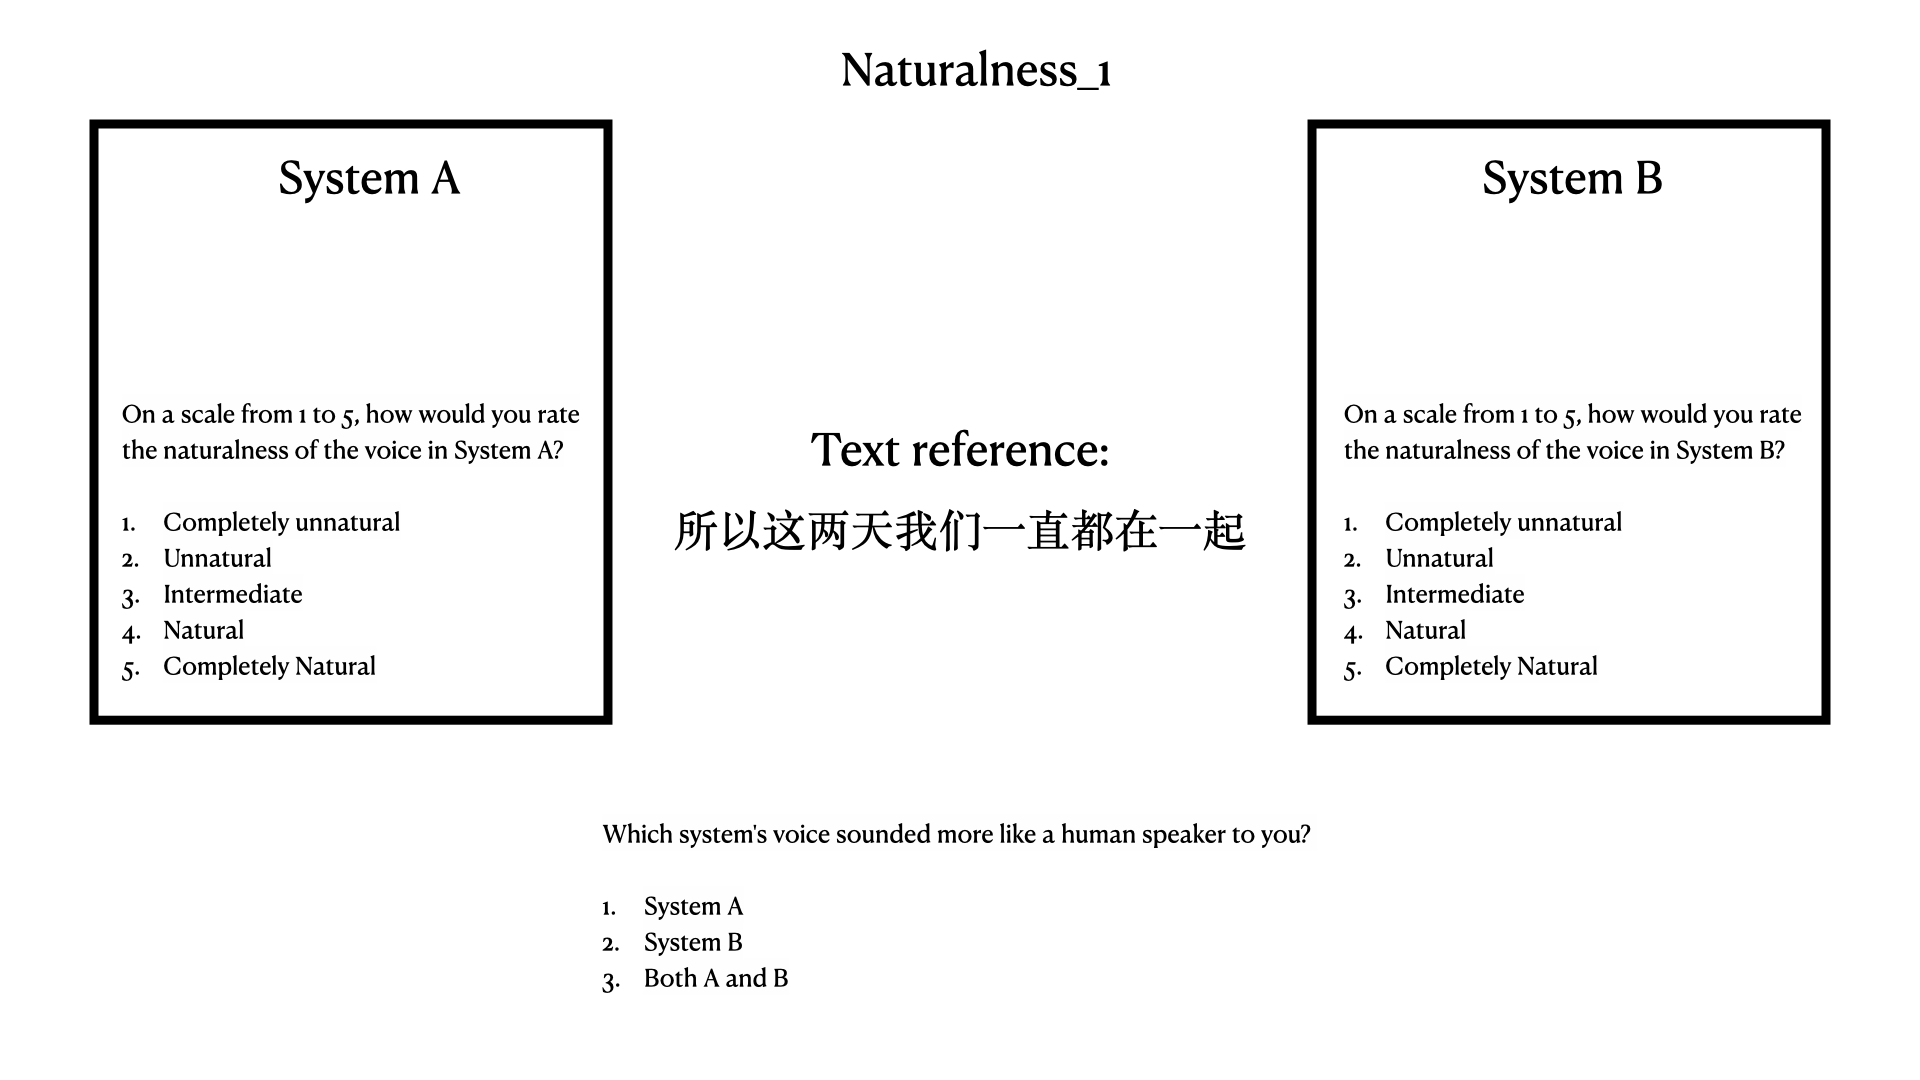
\includegraphics[width=0.5\textwidth]{demo_interface.001.png}
            \caption{Demo of Interface}
            \label{fig:my_label}
            \end{figure}
        \item Test Size:\\The test will consist of 40 audio samples in total. This will be divided into 5 sets for each aspect of evaluation (naturalness, intelligibility, emotion recognition, accent, and intonation), with each set containing 2 audio samples from each TTS system for direct comparison.
        \item Within-Subject Design:\\All listeners will hear exactly the same stimuli to ensure that each system is evaluated under the same conditions. The order of stimuli will be randomized for each listener to control for order effects and fatigue bias, ensuring that the position in the sequence does not unduly influence the listener's judgment.
        \item Rational: \\The chosen design aims to balance thoroughness with listener fatigue management. Forty audio samples are enough to cover a wide range of scenarios without overwhelming the listeners. Randomizing the order of presentation mitigates the risk of the listeners' responses being influenced by the sequence rather than the content. The side-by-side comparison facilitates a direct and clear understanding of the relative merits of each system.
    \end{itemize}
    \item The materials (stimuli) we use. \\We use “normal” materials, which are the segments of Mandarin from Chinese movies. At the same time, these segments exhibit significant emotional fluctuations.
    \item The number and categories of listeners we consider recruiting. \\For this task, we plan to recruit 500 listeners to ensure the reliability and generalizability of the results. Our listeners will primarily consist of Cantonese native speakers from the areas near Hong Kong and Guangzhou, who are also required to understand Mandarin. Within this broad category, we will further divide the listeners into two groups. The first is the general listeners who do not have a professional background in voice processing and can provide a general public perception of the TTS voice. The second group is the professional listeners, who have some understanding of voice processing and can provide a more professional and in-depth analysis.
    \item presentation: \\ You can access the demonstration through the following link \href{https://rug.eu.qualtrics.com/jfe/form/SV_0BtqBuja5LqE2vc}{Survey Link}. However, since Qualtrics doesn't support audio insertion, we have prepared a PowerPoint for further demonstration, which you can find in the attachment.
    \item Speech Dataset Credit to: \\ Chenye Cui, Yi Ren, Jinglin Liu, Feiyang Chen, Rongjie Huang, Ming Lei, Zhou Zhao from Zhejiang University and AlibabaGroup on \href{https://viem-ccy.github.io/EMOVIE/}{their website} and their thesis provide valuable insights, which you can find via the \href{https://arxiv.org/pdf/2106.09317.pdf}{link}

\end{enumerate}
\end{solution}


\end{document}
